\section{PVBall Class Reference}
\label{class_p_v_ball}\index{PVBall@{PVBall}}
Inherits {\bf PVNode}.

Collaboration diagram for PVBall:\nopagebreak
\begin{figure}[H]
\begin{center}
\leavevmode
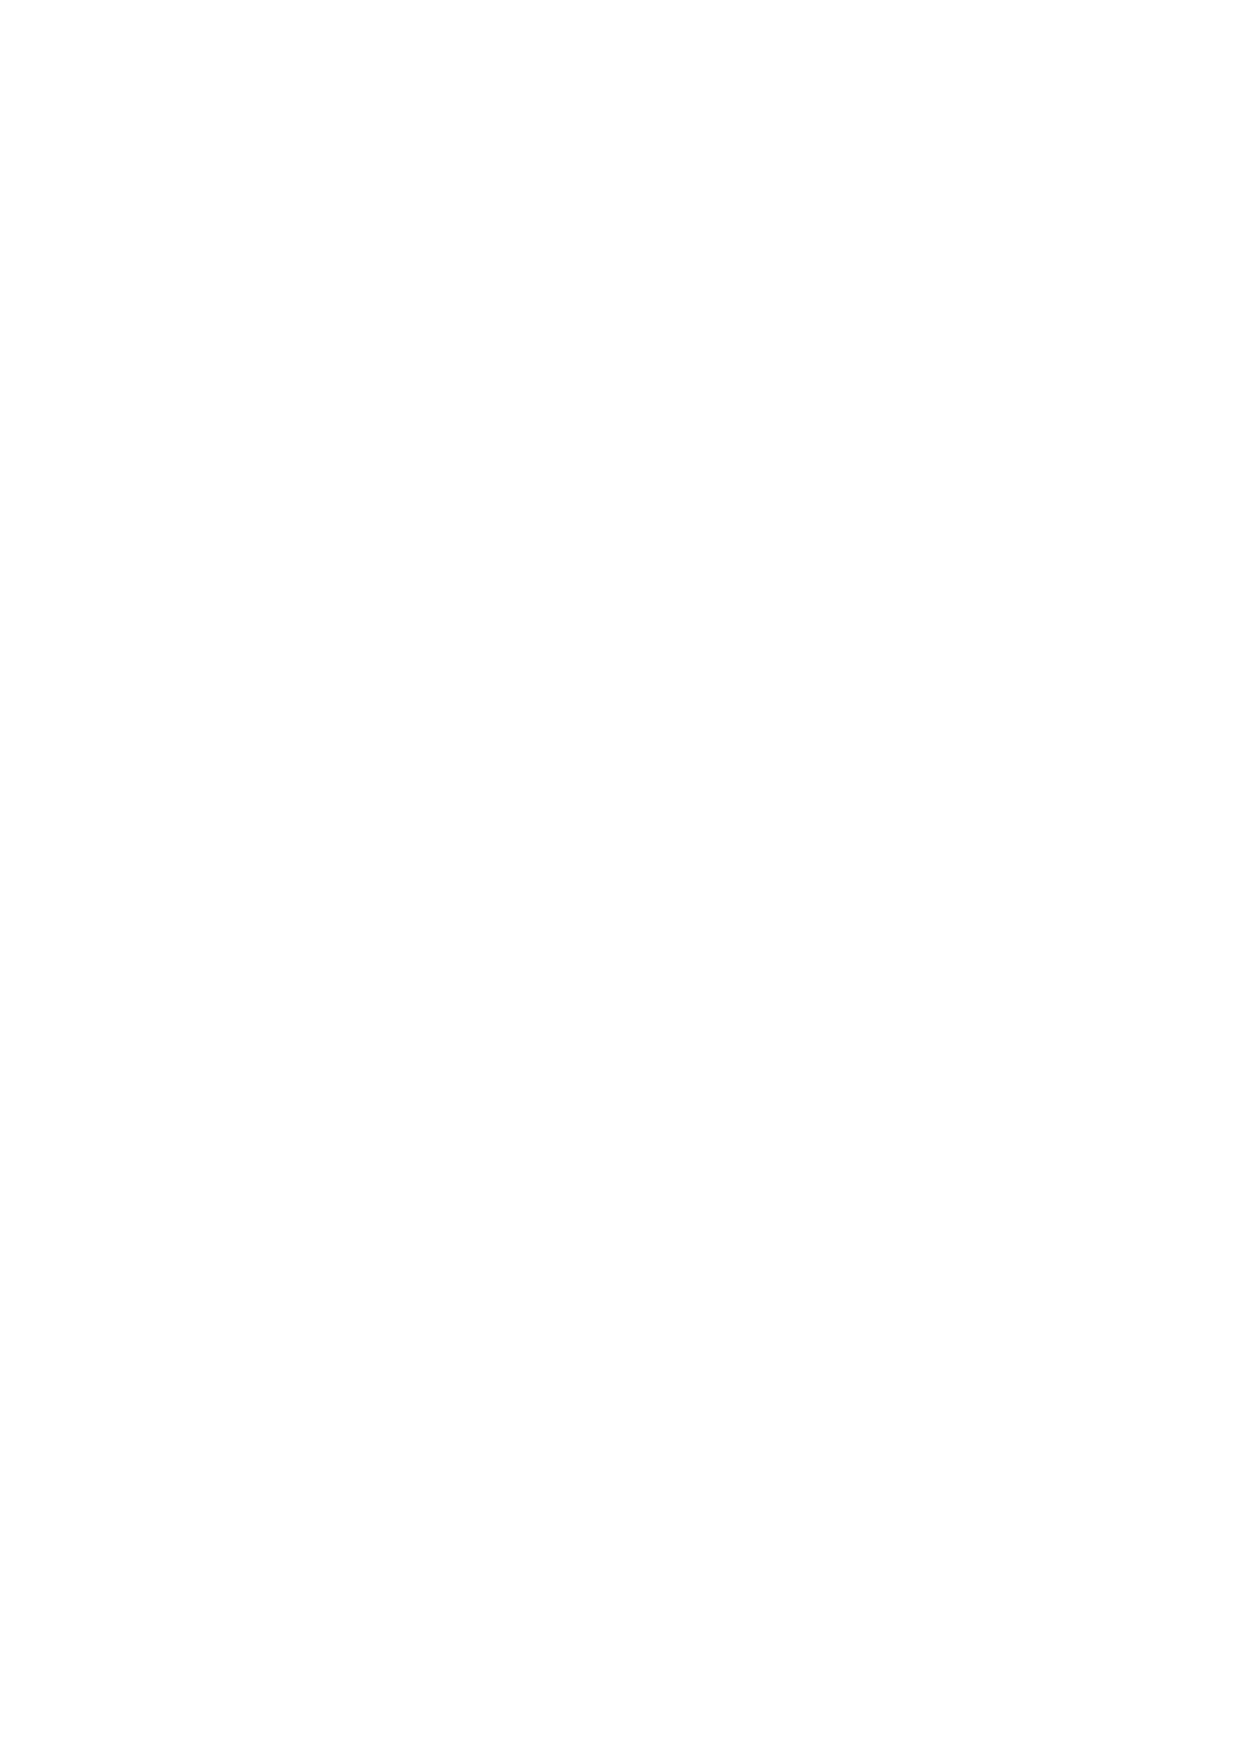
\includegraphics[width=44pt]{class_p_v_ball__coll__graph}
\end{center}
\end{figure}
\subsection*{Public Member Functions}
\begin{CompactItemize}
\item 
{\bf PVBall} ()
\item 
{\bf PVBall} (SceneNode $\ast$node, Entity $\ast$entity)
\item 
virtual {\bf $\sim$PVBall} ()
\item 
bool {\bf intersect} ()
\item 
int {\bf getId} ()
\item 
void {\bf setBallId} (int id)
\end{CompactItemize}
\subsection*{Static Public Member Functions}
\begin{CompactItemize}
\item 
static int {\bf getBallCount} ()
\end{CompactItemize}


\subsection{Constructor \& Destructor Documentation}
\index{PVBall@{PVBall}!PVBall@{PVBall}}
\index{PVBall@{PVBall}!PVBall@{PVBall}}
\subsubsection[{PVBall}]{\setlength{\rightskip}{0pt plus 5cm}PVBall::PVBall ()}\label{class_p_v_ball_86502630f0f62a9a51f7c51bf9519409}


\index{PVBall@{PVBall}!PVBall@{PVBall}}
\index{PVBall@{PVBall}!PVBall@{PVBall}}
\subsubsection[{PVBall}]{\setlength{\rightskip}{0pt plus 5cm}PVBall::PVBall (SceneNode $\ast$ {\em node}, \/  Entity $\ast$ {\em entity})}\label{class_p_v_ball_12ef7c87d000beae278975193872de49}


\index{PVBall@{PVBall}!$\sim$PVBall@{$\sim$PVBall}}
\index{$\sim$PVBall@{$\sim$PVBall}!PVBall@{PVBall}}
\subsubsection[{$\sim$PVBall}]{\setlength{\rightskip}{0pt plus 5cm}PVBall::$\sim$PVBall ()\hspace{0.3cm}{\tt  [virtual]}}\label{class_p_v_ball_a00806c0b3ea8703fd8f3882baa75a7d}




\subsection{Member Function Documentation}
\index{PVBall@{PVBall}!intersect@{intersect}}
\index{intersect@{intersect}!PVBall@{PVBall}}
\subsubsection[{intersect}]{\setlength{\rightskip}{0pt plus 5cm}bool PVBall::intersect ()}\label{class_p_v_ball_f9a225f53d94a8bf804e260d10ec34ee}


\index{PVBall@{PVBall}!getId@{getId}}
\index{getId@{getId}!PVBall@{PVBall}}
\subsubsection[{getId}]{\setlength{\rightskip}{0pt plus 5cm}int PVBall::getId ()}\label{class_p_v_ball_ba4d460f5a7d8e3741e9ab2f438157ca}


\index{PVBall@{PVBall}!setBallId@{setBallId}}
\index{setBallId@{setBallId}!PVBall@{PVBall}}
\subsubsection[{setBallId}]{\setlength{\rightskip}{0pt plus 5cm}void PVBall::setBallId (int {\em id})}\label{class_p_v_ball_5302c6790e1ac845b98c93b44d2dc5e4}


\index{PVBall@{PVBall}!getBallCount@{getBallCount}}
\index{getBallCount@{getBallCount}!PVBall@{PVBall}}
\subsubsection[{getBallCount}]{\setlength{\rightskip}{0pt plus 5cm}static int PVBall::getBallCount ()\hspace{0.3cm}{\tt  [static]}}\label{class_p_v_ball_7eb5352c9f20854605387107be0552e3}




The documentation for this class was generated from the following files:\begin{CompactItemize}
\item 
PVBall.h\item 
PVBall.cpp\end{CompactItemize}
